\chapter{Misura di resistenze con un multimetro digitale}\label{ch:mult}
    \lettrine[loversize=0.08, lines=2]{T}{ra le esperienze} svolte con il multimetro digitale riporto la misura delle resistenze di alcuni materiali, tra cui anelli metallici, il corpo umano e alcuni resistori.

    Ai resistori dedico una sezione più approfondita in quanto ho preso \num{50} misure su resistori distinti---ma teoricamente con resistenza uguale---per verificare la distribuzione delle misure di resistenza.

    \section{Il multimetro}
        Lo strumento utilizzato per l'interezza dell'esperienza è un multimetro digitale della serie \emph{DVM841} della \emph{Velleman\textsuperscript{\textregistered}} \cite{velleman-dvm841}. Il multimetro è in grado di misurare tensione e corrente continua e alternata, resistenza, frequenza e temperatura. Avendo una risoluzione di \num{2000} punti, il display del multimetro può visualizzare un massimo di \num{1999} unità.
    \section{Resistori}
        Il kit presenta \num{50} resistori distinti---come quelli in \figref{fig:mul:resistore}---il cui codice colore restituisce un valore\footnote{Lo si può dedurre da qualunque legenda fedele allo standard IEC 60062.} teorico di $\SI{820}{\ohm} \pm \SI{5}{\%}$, ovvero \SI{820(40)}{\ohm}.
        \begin{figure}
            \centering
            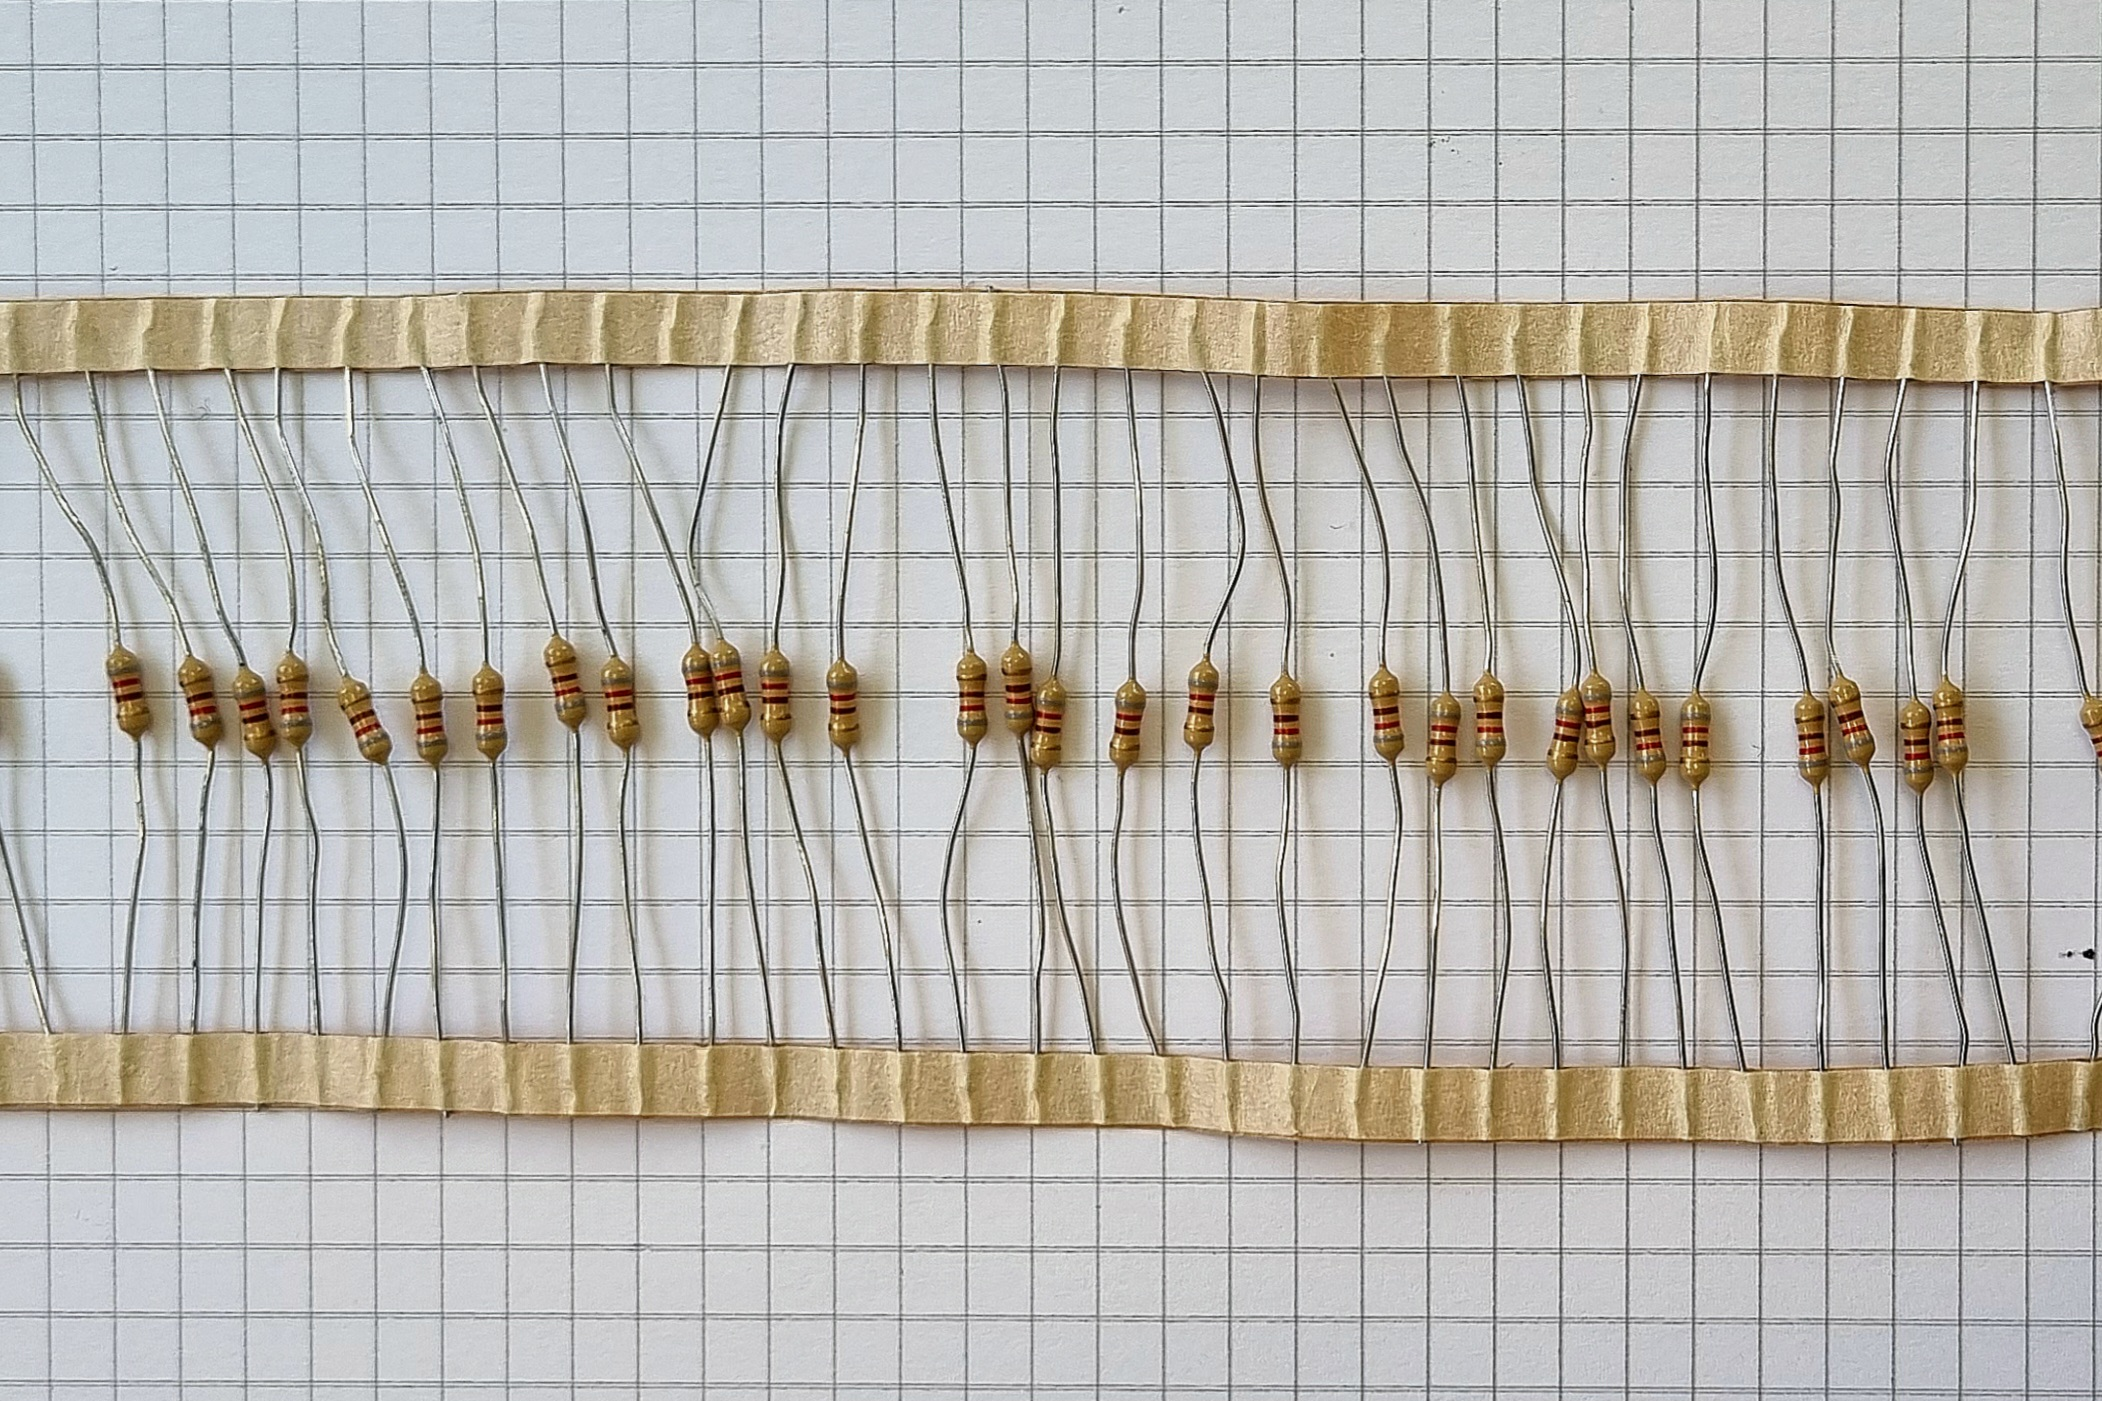
\includegraphics[width=0.4\textwidth]{images/multimetro/resistori.jpg}
            \hspace{0.05\textwidth}
            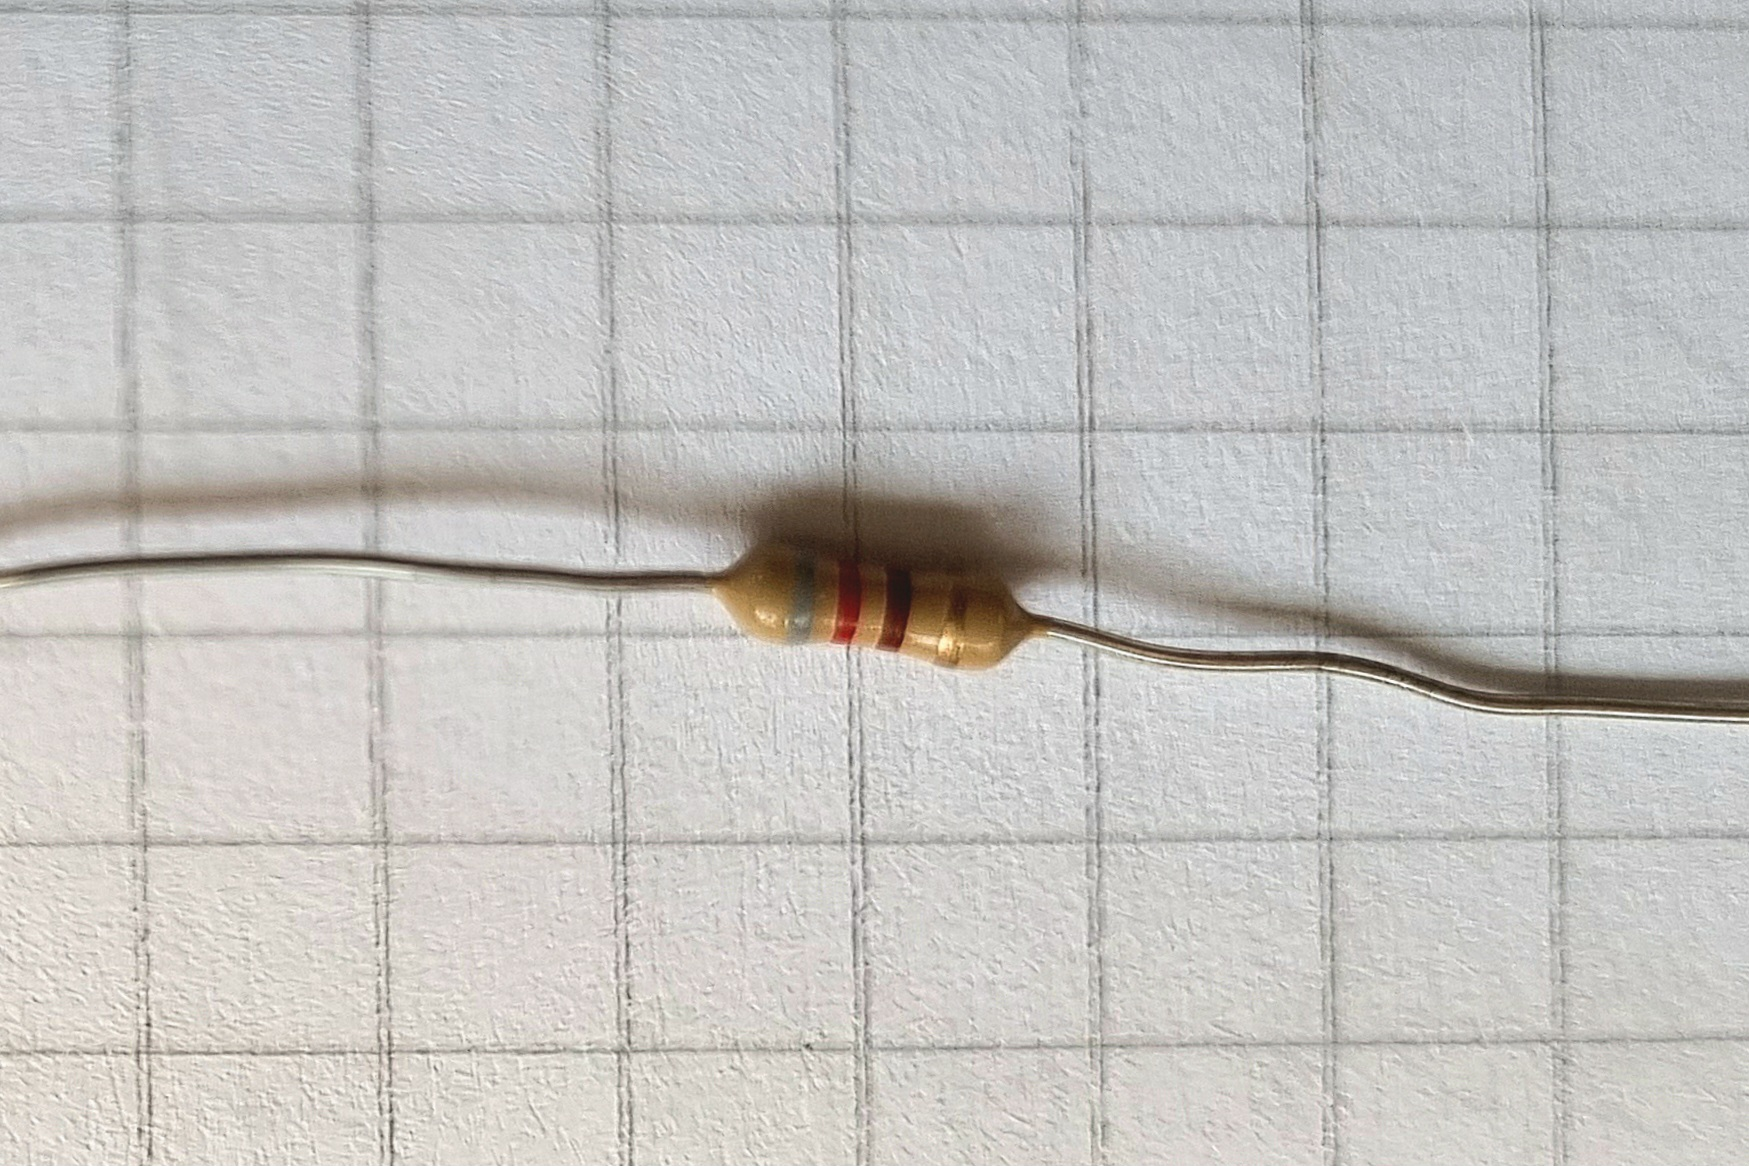
\includegraphics[width=0.4\textwidth]{images/multimetro/resistore.jpg}
            \caption{A sinistra alcuni dei \num{50} resistori da \SI{820}{\ohm}. A destra un dettaglio dove è visibile il codice colore.}
            \label{fig:mul:resistore}
        \end{figure}

        Ho effettuato le misure impostando il multimetro in modalità \emph{ohm}, alla portata di \SI{2}{\kilo\ohm}, poggiando i puntali sui terminali di ciascun resistore e aspettando di volta in volta che la lettura si stabilizzasse. I dati raccolti sono riportati in ordine crescente in \tabref{tab:mul:resistori}.
        \begin{table}
            \centering
            \begin{tabular}{cccccccccc}
    \hline
    \multicolumn{10}{c}{Resistenze (\unit{\ohm})}\\\hline\hline
    797 & 806 & 806 & 807 & 807 & 807 & 807 & 807 & 807 & 807 \\
    807 & 808 & 808 & 808 & 808 & 808 & 808 & 808 & 808 & 808 \\
    808 & 808 & 808 & 809 & 809 & 809 & 809 & 809 & 809 & 809 \\
    809 & 809 & 809 & 809 & 809 & 809 & 810 & 810 & 810 & 810 \\
    810 & 810 & 810 & 811 & 811 & 812 & 812 & 812 & 812 & 813 \\ \hline
\end{tabular}
            \caption{Misure di resistenza effettuate su \num{50} resistori distinti.}
            \label{tab:mul:resistori}
        \end{table}

        Notiamo subito che la resistenza media è $R_\text{m} = \SI{808.6}{\ohm}$ con una deviazione standard di $\sigma_R = \SI{2.3}{\ohm}$, valori che rientrano nell'intervallo fornito dal costruttore. Tuttavia, il fatto che tutte le singole misure siano inferiori a \SI{820}{\ohm} suggerisce la presenza di un errore sistematico---ad esempio una staratura dello strumento: se si trattasse di oscillazioni delle stesse resistenze dovute alla costruzione, mi aspetterei letture sia al di sopra che al di sotto del valore di riferimento; è poco probabile che tutte le resistenze devino dal valore teorico allo stesso modo.
        